\documentclass[../../../../dd.tex]{subfiles}

\begin{document}

	\section{High Level Components and Their Interaction}
		In this section each Tier is decomposed in his high level components. For each component is given a short description of his purpose and how the component interacts with the others components.
	
		\subfile{chapters/architecturalDesign/sections/highLevelComponentsAndTheirInteraction/subsections/dataTier/dataTier.tex}

		\subfile{chapters/architecturalDesign/sections/highLevelComponentsAndTheirInteraction/subsections/logicTier/logicTier.tex}

		\subfile{chapters/architecturalDesign/sections/highLevelComponentsAndTheirInteraction/subsections/presentationTier/presentationTier.tex}

		\subsection{Schema}
			For a description of what is written so far it's provided a schema of the systems

			\begin{figure}[H]
				\centering
				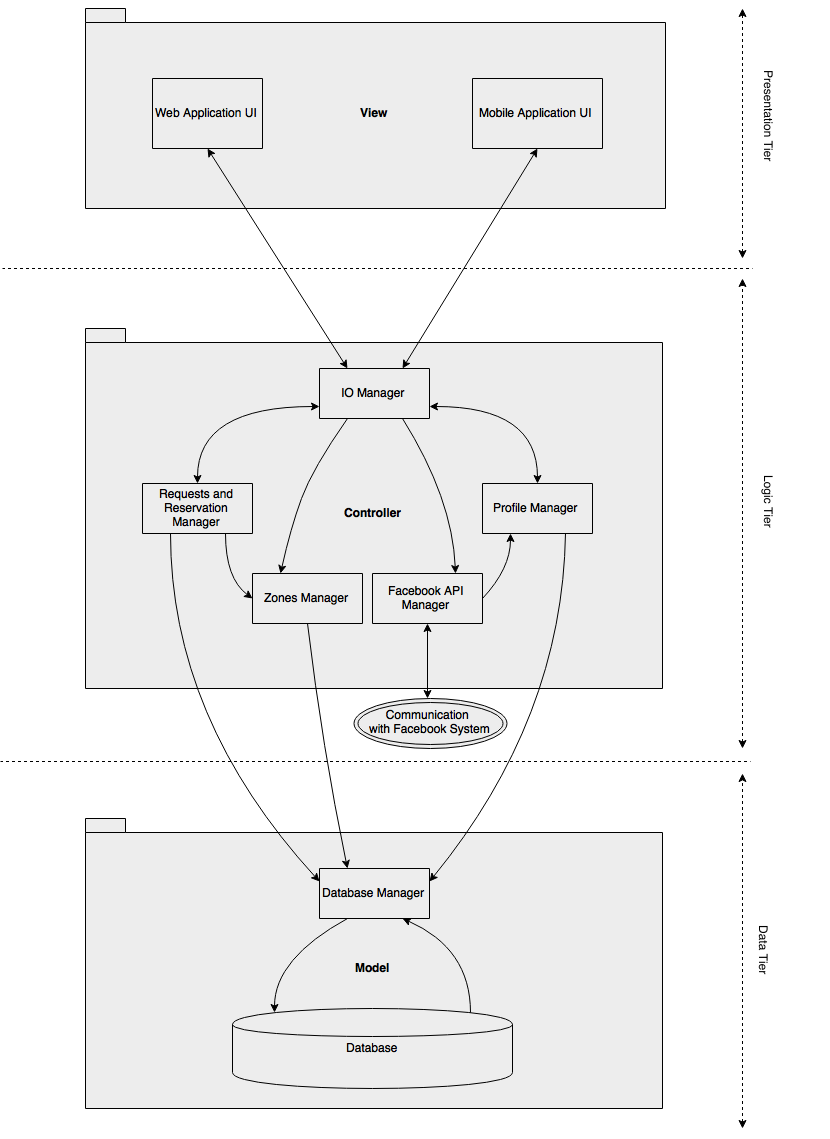
\includegraphics[width=\textwidth, scale=0.5]{../images/HighLevelComponents}
			\caption{High Level Components and Interactions}\label{fig:HighLevelComponents}
		\end{figure}
	
\end{document}